%==============================================================================
% PAPER 2, CHAPTER 1: Cayley-Dickson Algebras
%==============================================================================

\chapter{Cayley-Dickson Algebras: Beyond Complex Numbers}
\label{ch:p2:cayley-dickson}

\marginphysics{Electron spin requires quaternions; string theory requires octonions}

\section{The Spin Mystery: Why Quantum Mechanics Needs More Than Complex Numbers}

When physicists first discovered electron spin in the 1920s, complex numbers were not enough. A spinning electron does not behave like a rotating ball---it requires \emph{two} full rotations (720 degrees) to return to its original quantum state.\marginhistory{Stern-Gerlach experiment, 1922: First demonstration of spin quantization} One rotation by 360 degrees changes the wavefunction's sign.

This bizarre property demands a number system beyond the complex plane. Wolfgang Pauli solved the puzzle with his famous spin matrices:
\begin{equation}
  \sigma_x = \begin{pmatrix} 0 & 1 \\ 1 & 0 \end{pmatrix}, \quad
  \sigma_y = \begin{pmatrix} 0 & -i \\ i & 0 \end{pmatrix}, \quad
  \sigma_z = \begin{pmatrix} 1 & 0 \\ 0 & -1 \end{pmatrix}
  \label{eq:p2:cayley:pauli-intro}
\end{equation}

These matrices satisfy $\sigma_i \sigma_j = i\epsilon_{ijk} \sigma_k$.\marginmath{Levi-Civita tensor $\epsilon_{ijk}$ encodes cross product} But there's a deeper pattern: these are the imaginary units of \textbf{quaternions}---the four-dimensional number system discovered by William Rowan Hamilton in 1843.

Hamilton famously carved the quaternion multiplication rules into a bridge in Dublin:\marginhistory{Brougham Bridge, Dublin, October 16, 1843}
\begin{equation}
  i^2 = j^2 = k^2 = ijk = -1
  \label{eq:p2:cayley:hamilton-carving}
\end{equation}

But nature does not stop at four dimensions. String theory requires ten dimensions. M-theory requires eleven. Grand unified theories embed the Standard Model in exceptional Lie groups living in 78, 133, or 248 dimensions.\marginphysics{Standard Model fits inside $E_6$ (78D) or $E_8$ (248D)}

\textbf{How do we build number systems for these higher dimensions?} The answer is the Cayley-Dickson construction: a recursive doubling process that generates $2^n$-dimensional algebras from one-dimensional real numbers up to 2048 dimensions and beyond.

Here's the remarkable fact: \textbf{every doubling costs us an algebraic property}.\margincaution{Loss of structure enables richer physics}
\begin{itemize}
  \item After $\mathbb{C}$ (2D): Commutativity lost. $ij \neq ji$.
  \item After $\mathbb{H}$ (4D): Associativity lost. $(xy)z \neq x(yz)$.
  \item After $\mathbb{O}$ (8D): Division algebra property lost. Zero divisors appear.
\end{itemize}

\section{The Doubling Principle}
\label{sec:p2:cayley:construction}

\subsection{Motivation: Why Pairs?}

The clever insight: \textbf{treat elements of the new algebra as ordered pairs} from the old algebra.\marginmath{Ordered pairs $(a,b)$ create next dimension} This is exactly how we construct complex numbers from reals:
\begin{equation}
  z = a + bi = (a, b) \quad \text{where } a, b \in \mathbb{R}
\end{equation}

Complex multiplication $(a_1, b_1) \cdot (a_2, b_2) = (a_1 a_2 - b_1 b_2, a_1 b_2 + a_2 b_1)$ emerges from $i^2 = -1$.\margincomp{Check: $(0,1)(0,1) = (-1,0)$}

\subsection{The Recursive Hierarchy}

Starting from $\mathbb{R}$ (1D), each doubling creates a new algebra:\marginphysics{Each algebra has distinct physical applications}
\begin{equation}
  \mathbb{R} \xrightarrow{2D} \mathbb{C} \xrightarrow{4D} \mathbb{H} \xrightarrow{8D} \mathbb{O} \xrightarrow{16D} \mathbb{S} \xrightarrow{32D} \mathbb{P}
\end{equation}

\textbf{The algebras}:
\begin{itemize}
  \item $\mathbb{R}$ (1D): Real numbers
  \item $\mathbb{C}$ (2D): Complex numbers
  \item $\mathbb{H}$ (4D): Quaternions (Hamilton, 1843)
  \item $\mathbb{O}$ (8D): Octonions (Graves/Cayley, 1845)
  \item $\mathbb{S}$ (16D): Sedenions
  \item $\mathbb{P}$ (32D): Pathions
\end{itemize}

At each step, the dimension doubles: $\dim(\mathcal{A}_{n+1}) = 2 \cdot \dim(\mathcal{A}_n)$.

\begin{figure}[htbp]
\centering
\begin{tikzpicture}[
  node distance=2.5cm,
  algebra/.style={rectangle, rounded corners, draw=blue!70, fill=blue!10, thick, minimum height=1.2cm, minimum width=1.8cm, align=center, font=\small},
  arrow/.style={->, >=stealth, thick, blue!70},
  loss/.style={font=\tiny, red!70!black, align=center}
]
  % Algebras
  \node[algebra] (R) {$\mathbb{R}$\\1D\\Reals};
  \node[algebra, right of=R] (C) {$\mathbb{C}$\\2D\\Complex};
  \node[algebra, right of=C] (H) {$\mathbb{H}$\\4D\\Quaternions};
  \node[algebra, right of=H] (O) {$\mathbb{O}$\\8D\\Octonions};
  \node[algebra, below=1.5cm of H] (S) {$\mathbb{S}$\\16D\\Sedenions};
  \node[algebra, below=1.5cm of O] (P) {$\mathbb{P}$\\32D\\Pathions};

  % Arrows with doubling
  \draw[arrow] (R) -- (C) node[midway, above, font=\footnotesize] {$\times 2$};
  \draw[arrow] (C) -- (H) node[midway, above, font=\footnotesize] {$\times 2$};
  \draw[arrow] (H) -- (O) node[midway, above, font=\footnotesize] {$\times 2$};
  \draw[arrow] (O) -- (S) node[midway, right, font=\footnotesize] {$\times 2$};
  \draw[arrow] (S) -- (P) node[midway, below, font=\footnotesize] {$\times 2$};

  % Property losses
  \node[loss, below=0.1cm of R] {};
  \node[loss, below=0.1cm of C] {Lost:\\Ordering};
  \node[loss, below=0.1cm of H] {Lost:\\Commutativity};
  \node[loss, below=0.3cm of O] {Lost:\\Associativity};
  \node[loss, right=0.1cm of S] {Lost:\\Division\\Zero divisors};
  \node[loss, right=0.1cm of P] {Lost:\\Alternativity};

  % Title annotation
  \node[draw=none, font=\footnotesize\bfseries, above=0.8cm of C] {Cayley-Dickson Doubling Progression};

  % Recursive formula box
  \node[draw=green!60!black, fill=green!5, thick, rounded corners, align=left, font=\scriptsize, below=0.5cm of S, xshift=-1cm] {
    \textbf{Doubling formula:}\\
    $(a,b) \cdot (c,d) = (ac - d^*b, da + bc^*)$\\
    Dimension: $2^{n+1}$ from $2^n$
  };

\end{tikzpicture}
\caption{Cayley-Dickson recursion showing dimensional doubling from reals to pathions. Each doubling (blue arrows) doubles the dimension but costs an algebraic property (red labels). The construction terminates practical usefulness at octonions (8D), the last normed division algebra, though it can continue indefinitely. The green box shows the universal multiplication rule generating all algebras.}
\label{fig:p2:cayley:recursion}
\end{figure}

\marginxref{Fig.~\ref{fig:p2:cayley:recursion}: Doubling hierarchy}

\subsection{The Universal Multiplication Rule}

Elements of $\mathcal{A}_{n+1}$ are pairs $(a,b)$ with $a,b \in \mathcal{A}_n$:\marginmath{Single formula generates all algebras}
\begin{equation}
  (a,b) \cdot (c,d) = (ac - d^* b, da + bc^*)
  \label{eq:p2:cayley:formula}
\end{equation}

The conjugation operation is recursive: $(a,b)^* = (a^*, -b)$.

\subsection{Norm Preservation}

The quadratic norm is:\marginphysics{Norm-squared = Probability density in QM}
\begin{equation}
  \|x\|^2 = x \cdot x^* = \sum_{i=1}^{2^n} x_i^2
\end{equation}

For algebras through pathions (32D), the norm is multiplicative:\marginmath{$\|xy\| = \|x\|\,\|y\|$ through 32D}
\begin{equation}
  \|xy\| = \|x\|\,\|y\|
\end{equation}

\textbf{Physical consequence}: Probability conservation in quantum mechanics.

\section{The Classical Division Algebras}

\subsection{Real Numbers $\mathbb{R}$ (1D)}

All desirable properties:\marginmath{Commutative + Associative + Division}
\begin{itemize}
  \item Commutative: $ab = ba$
  \item Associative: $(ab)c = a(bc)$
  \item Division algebra: $ab = 0 \implies a=0$ or $b=0$
  \item Normed: $|ab| = |a|\,|b|$
\end{itemize}

\subsection{Complex Numbers $\mathbb{C}$ (2D)}

Complex numbers $z = a + bi$ with $i^2 = -1$.\marginphysics{Quantum interference requires complex amplitudes}

\textbf{Worked example}: $(3 + 4i)(1 + 2i)$:\marginex{Standard FOIL expansion}
\begin{align}
  (3 + 4i)(1 + 2i) &= 3 + 6i + 4i + 8i^2 \nonumber \\
  &= 3 + 10i - 8 = -5 + 10i
\end{align}

Check norm: $|3+4i| = 5$, $|1+2i| = \sqrt{5}$, $|-5+10i| = 5\sqrt{5}$. Indeed $5 \cdot \sqrt{5} = 5\sqrt{5}$.\margincomp{Norm multiplicativity verified}

\subsection{Quaternions $\mathbb{H}$ (4D)}

Quaternions $q = a + bi + cj + dk$ with three imaginary units:\marginmath{Three units: $i, j, k$}
\begin{equation}
  i^2 = j^2 = k^2 = ijk = -1
\end{equation}

Multiplication table:\marginphysics{Non-commutative: $ij = k \neq ji = -k$}
\begin{equation}
  \begin{array}{c|cccc}
    \cdot & 1 & i & j & k \\
    \hline
    1 & 1 & i & j & k \\
    i & i & -1 & k & -j \\
    j & j & -k & -1 & i \\
    k & k & j & -i & -1
  \end{array}
\end{equation}

\textbf{Worked example}: $(1 + i)(j + k) = j + k + k - j = 2k$\marginex{Expand using distributive law}

Reverse order: $(j + k)(1 + i) = j - k + k + j = 2j$. Different results!\margincaution{Non-commutativity at 4D}

\textbf{Physical significance}: Quaternions describe 3D rotations.\marginphysics{3D rotations → Unit quaternions} A rotation by angle $\theta$ about axis $\mathbf{n}$ is:
\begin{equation}
  q = \cos(\theta/2) + \sin(\theta/2)(n_x i + n_y j + n_z k)
\end{equation}

Rotating vector $\mathbf{v}$: $\mathbf{v}' = q \mathbf{v} q^{-1}$.\margincomp{More efficient than $3 \times 3$ matrices}

The Pauli spin matrices are quaternion units in disguise.\marginphysics{Electron spin → Quaternionic structure}

\begin{figure}[htbp]
\centering
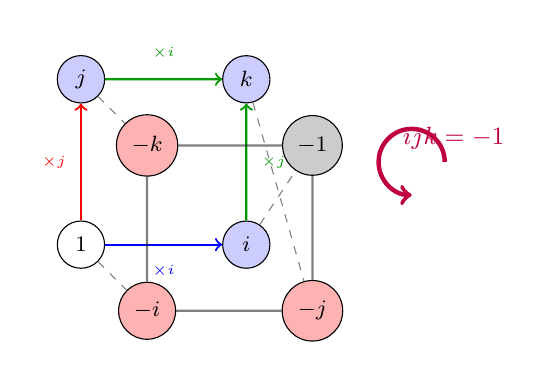
\begin{tikzpicture}[scale=1.4, every node/.style={circle, draw, fill=blue!20, minimum size=6mm, font=\footnotesize}]
  % Define quaternion unit positions at vertices of a cube projection
  \def\cubescale{1.5}
  % Front face (z=0 plane)
  \node[fill=white] (1) at (0,0) {$1$};
  \node (i) at (\cubescale,0) {$i$};
  \node (j) at (0,\cubescale) {$j$};
  \node (k) at (\cubescale,\cubescale) {$k$};
  % Back face (z=1 plane)
  \node[fill=red!30] (ni) at (0.4*\cubescale,-0.4*\cubescale) {$-i$};
  \node[fill=red!30] (nj) at (0.4*\cubescale+\cubescale,-0.4*\cubescale) {$-j$};
  \node[fill=red!30] (nk) at (0.4*\cubescale,\cubescale-0.4*\cubescale) {$-k$};
  \node[fill=gray!40] (n1) at (0.4*\cubescale+\cubescale,\cubescale-0.4*\cubescale) {$-1$};

  % Edges showing multiplication paths (color-coded for clarity)
  \draw[thick, blue, ->] (1) -- (i) node[midway, below, draw=none, fill=none] {\tiny $\times i$};
  \draw[thick, red, ->] (1) -- (j) node[midway, left, draw=none, fill=none] {\tiny $\times j$};
  \draw[thick, green!60!black, ->] (i) -- (k) node[midway, right, draw=none, fill=none] {\tiny $\times j$};
  \draw[thick, green!60!black, ->] (j) -- (k) node[midway, above, draw=none, fill=none] {\tiny $\times i$};

  % Diagonal edges (depth)
  \draw[dashed, gray] (1) -- (ni);
  \draw[dashed, gray] (i) -- (n1);
  \draw[dashed, gray] (j) -- (nk);
  \draw[dashed, gray] (k) -- (nj);

  % Back face edges
  \draw[thick, opacity=0.5] (ni) -- (nj);
  \draw[thick, opacity=0.5] (ni) -- (nk);
  \draw[thick, opacity=0.5] (nj) -- (n1);
  \draw[thick, opacity=0.5] (nk) -- (n1);

  % Cyclic multiplication: ijk = -1
  \draw[ultra thick, purple, ->] (2.2*\cubescale, 0.5*\cubescale) arc (0:270:0.3) node[midway, right, draw=none, fill=none, font=\small] {$ijk = -1$};
\end{tikzpicture}
\caption{Quaternion multiplication cube showing the three imaginary units $i, j, k$ and their negatives. The colored arrows indicate multiplication paths: $ij = k$ (green), $jk = i$ (blue), $ki = j$ (red). Non-commutativity is evident: $ij = k$ but $ji = -k$. The cyclic relation $ijk = -1$ (purple) is Hamilton's fundamental quaternion identity.}
\label{fig:p2:cayley:quaternion-cube}
\end{figure}

\marginxref{Fig.~\ref{fig:p2:cayley:quaternion-cube}: Quaternion structure in 3D}

\subsection{Octonions $\mathbb{O}$ (8D)}

Octonions are eight-dimensional with basis $\{1, e_1, \ldots, e_7\}$. The seven imaginary units multiply via the \textbf{Fano plane}.\marginmath{Fano plane: 7 points, 7 lines}

\textbf{Non-associativity}: $(e_1 e_2) e_4 \neq e_1 (e_2 e_4)$.\margincaution{Associativity lost at 8D}

Using the Fano plane:\marginex{Products from Fano geometry}
\begin{align}
  (e_1 e_2) e_4 &= e_3 e_4 = e_6 \\
  e_1 (e_2 e_4) &= e_1 e_7 = -e_5
\end{align}

Since $e_6 \neq -e_5$, associativity fails.\marginmath{Grouping matters: $(xy)z \neq x(yz)$}

Octonions satisfy the weaker \textbf{Moufang identities}: $x(xy) = (xx)y$ and $(yx)x = y(xx)$.\marginmath{Alternative algebra: Moufang identities}

\begin{figure}[htbp]
\centering
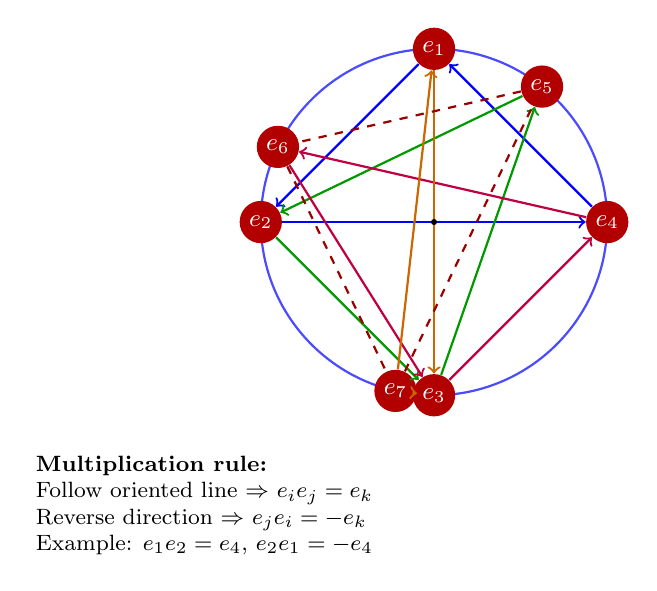
\begin{tikzpicture}[scale=2.2]
  % Fano plane circle
  \draw[thick, blue!70] (0,0) circle (1);

  % Seven vertices (imaginary units e1-e7)
  \foreach \i/\angle/\label in {1/90/e_1, 2/180/e_2, 3/270/e_3, 4/360/e_4, 5/51.43/e_5, 6/154.29/e_6, 7/257.14/e_7} {
    \node[circle, fill=red!70!black, inner sep=2pt, text=white, font=\small] (\i) at (\angle:1) {$\label$};
  }

  % Seven lines (with orientation arrows for multiplication)
  % Line 1: e1-e2-e4 (triangle side)
  \draw[thick, blue, ->] (1) -- (2);
  \draw[thick, blue, ->] (2) -- (4);
  \draw[thick, blue, ->] (4) -- (1);

  % Line 2: e2-e3-e5 (triangle side)
  \draw[thick, green!60!black, ->] (2) -- (3);
  \draw[thick, green!60!black, ->] (3) -- (5);
  \draw[thick, green!60!black, ->] (5) -- (2);

  % Line 3: e3-e4-e6 (triangle side)
  \draw[thick, purple, ->] (3) -- (4);
  \draw[thick, purple, ->] (4) -- (6);
  \draw[thick, purple, ->] (6) -- (3);

  % Line 4: e1-e3-e7 (through center)
  \draw[thick, orange!80!black, ->] (1) -- (3);
  \draw[thick, orange!80!black, ->] (3) -- (7);
  \draw[thick, orange!80!black, ->] (7) -- (1);

  % Central triangle (inscribed)
  \draw[thick, red!60!black, dashed] (5) -- (6);
  \draw[thick, red!60!black, dashed] (6) -- (7);
  \draw[thick, red!60!black, dashed] (7) -- (5);

  % Center point
  \fill[black] (0,0) circle (0.5pt);

  % Legend for multiplication rule
  \node[draw=none, fill=white, align=left, font=\footnotesize, below left, inner sep=3pt] at (-0.3,-1.3) {
    \textbf{Multiplication rule:}\\
    Follow oriented line $\Rightarrow$ $e_i e_j = e_k$\\
    Reverse direction $\Rightarrow$ $e_j e_i = -e_k$\\
    Example: $e_1 e_2 = e_4$, $e_2 e_1 = -e_4$
  };
\end{tikzpicture}
\caption{Fano plane encoding octonion multiplication. Seven imaginary units $e_1, \ldots, e_7$ sit at the vertices. Seven lines (including the circle and central triangle) each contain three units. Following the arrow direction from $e_i$ to $e_j$ to $e_k$ gives $e_i e_j = e_k$. Reversing gives a sign flip: $e_j e_i = -e_k$. Non-associativity arises from cyclic permutations not preserving products.}
\label{fig:p2:cayley:fano-plane}
\end{figure}

\marginxref{Fig.~\ref{fig:p2:cayley:fano-plane}: Fano plane multiplication}

\textbf{Hurwitz theorem} (1898): $\mathbb{R}, \mathbb{C}, \mathbb{H}, \mathbb{O}$ are the \emph{only} normed division algebras.\marginhistory{Hurwitz: Only 1, 2, 4, 8 dimensions}

\textbf{Physical significance}:\marginphysics{Octonions → Exceptional symmetries}
\begin{itemize}
  \item Automorphism group is $G_2$ (smallest exceptional Lie group)
  \item Appear in $E_8 \times E_8$ heterotic string theory
  \item $\text{Spin}(8)$ triality connects vector/spinor representations
\end{itemize}

\section{Beyond Division Algebras}

\subsection{Sedenions $\mathbb{S}$ (16D)}

Sedenions contain \textbf{zero divisors}: non-zero $a, b$ with $ab = 0$.\margincaution{Zero divisors at 16D}

\textbf{Physical interpretation}: Zero divisors correspond to topological defects:\marginphysics{$ab = 0$ → Topological defects}
\begin{itemize}
  \item Cosmic strings (line defects)
  \item Monopoles (point defects)
  \item Domain walls (surface defects)
\end{itemize}

Properties lost:\marginmath{Non-alternative, not a division algebra}
\begin{itemize}
  \item Non-alternative
  \item Not a division algebra
  \item Contains zero divisors
\end{itemize}

\subsection{Pathions $\mathbb{P}$ (32D)}

Pathions (32D) connect to supersymmetry:\marginphysics{32D → Maximal supersymmetry}
\begin{itemize}
  \item $\mathcal{N}=8$ supergravity has 32 supercharges
  \item $E_8 \times E_8$ heterotic strings (rank 16 + 16 = 32)
\end{itemize}

\section{Systematic Loss of Structure}

\begin{table}[htb]
\centering
\caption{Properties of Cayley-Dickson algebras}
\begin{tabular}{lcccccc}
\toprule
Algebra & Dim & Commutative & Associative & Alternative & Division & Normed \\
\midrule
$\mathbb{R}$ & 1 & \checkmark & \checkmark & \checkmark & \checkmark & \checkmark \\
$\mathbb{C}$ & 2 & \checkmark & \checkmark & \checkmark & \checkmark & \checkmark \\
$\mathbb{H}$ & 4 & \texttimes & \checkmark & \checkmark & \checkmark & \checkmark \\
$\mathbb{O}$ & 8 & \texttimes & \texttimes & \checkmark & \checkmark & \checkmark \\
$\mathbb{S}$ & 16 & \texttimes & \texttimes & \texttimes & \texttimes & semi \\
$\mathbb{P}$ & 32 & \texttimes & \texttimes & \texttimes & \texttimes & semi \\
\bottomrule
\end{tabular}
\end{table}

\marginhistory{Frobenius (1878): Only $\mathbb{R}, \mathbb{C}, \mathbb{H}$ are associative division algebras}

\section{Connections to Exceptional Lie Groups}

The Cayley-Dickson algebras connect to exceptional Lie groups:

\subsection{$G_2$: Octonion Automorphisms}

$G_2$ is the automorphism group of octonions:\marginmath{$G_2 = \text{Aut}(\mathbb{O})$}
\begin{equation}
  G_2 = \{ g \in \text{GL}(7,\mathbb{R}) \mid g(xy) = g(x)g(y) \}
\end{equation}

Dimension: 14 (as a Lie group)\marginphysics{$G_2$ in M-theory compactifications}

\subsection{$E_8$: Hierarchical Structure}

The exceptional groups form a chain:\marginmath{$E_8 \supset E_7 \supset E_6 \supset F_4 \supset G_2$}
\begin{equation}
  E_8 \supset E_7 \supset E_6 \supset F_4 \supset G_2
\end{equation}

This parallels the Cayley-Dickson doubling hierarchy.\marginphysics{Heterotic strings: $E_8 \times E_8$}

\textbf{String theory}: $E_8 \times E_8$ heterotic strings arise from:
\begin{equation}
  T^{16} = \Lambda_{E_8} \oplus \Lambda_{E_8}
\end{equation}

\section{Summary}

We constructed the Cayley-Dickson tower from real numbers to high dimensions:

\textbf{Key results}:\marginxref{Next chapter: Exceptional Lie groups}
\begin{enumerate}
  \item Recursive doubling: $(a,b)(c,d) = (ac - d^*b, da + bc^*)$
  \item Classical division algebras: $\mathbb{R}, \mathbb{C}, \mathbb{H}, \mathbb{O}$ only
  \item Progressive structure loss at each doubling
  \item Connections to exceptional groups $G_2, F_4, E_6, E_7, E_8$
\end{enumerate}

\textbf{Forward bridge}: Chapter~\ref{ch:p2:exceptional-lie-groups} develops exceptional Lie groups in detail.

%==============================================================================
% END OF CHAPTER 1
%==============================================================================
